% !LW recipe=pdflatex
% !TEX root = tvuontis.tex
%% This file is modified by Jussi Kangasharju and Pirjo Moen.
%% Earlier versions were made by Veli Mäkinen
%% from HY_fysiikka_LuKtemplate.tex authored by Roope Halonen ja
%% Tomi Vainio. Some text is also inherited from engl_malli.tex by
%% Kutvonen, Erkiö, Mäkelä, Verkamo, Kurhila, and Nykänen.
%% 
%% 
% STEP 1: Choose oneside or twoside
\documentclass[english,oneside,openany]{UH_DS_report}
%finnish,swedish
%
%\usepackage[utf8]{inputenc} 
% For UTF8 support. Use UTF8 when saving your file.
\usepackage{lmodern} % Font package 
\usepackage{textcomp} % Package for special symbols 
\usepackage[pdftex]{color, graphicx} % For pdf output and jpg/png graphics 
\usepackage[pdftex, plainpages=false]{hyperref} % For hyperlinks and pdf metadata 
\usepackage{fancyhdr} % For nicer page headers 
\usepackage{tikz} % For making vector graphics (hard to learn but powerful)
%\usepackage{wrapfig} % For nice text-wrapping figures (use at own discretion)
\usepackage{amsmath, amssymb} % For better math
%\usepackage[square]{natbib} % For bibliography
\usepackage[footnotesize,bf]{caption} % For more control over figure captions 
\usepackage{blindtext} 
\usepackage{titlesec}
\usepackage[titletoc]{appendix}
\usepackage{cleveref}

\onehalfspacing %line spacing
%\singlespacing 
%\doublespacing

%\fussy 
\sloppy % sloppy and fussy commands can be used to avoid overlong text lines

% STEP 2: 
% Set up all the information for the title page and the abstract form. 
% Replace parameters with your information.
\title{VMBC Report} 
\author{Tuomas Vuontisjarvi}

\date{\today}
\keywords{} 
\depositeplace{}
\additionalinformation{}

% \classification{\protect{\ \\
%     \  General and reference $\rightarrow$ Document types $\rightarrow$ Surveys and overviews\  \\
%     \  Applied computing $\rightarrow$ Document management and text processing $\rightarrow$ Document management $\rightarrow$ Text editing\\
% }}

% If you want to quote someone special. You can comment this line and
% there will be nothing on the document.
%\quoting{Bachelor's degrees make pretty good placemats if you get them
%laminated.}{Jeph Jacques}

% OPTIONAL STEP: Set up properties and metadata for the pdf file that
% pdfLaTeX makes. But you don't really need to do this unless you want
% to.
\hypersetup{ 
	%bookmarks=true,         % show bookmarks bar first?
	unicode=true,           % to show non-Latin characters in Acrobat's bookmarks 
	pdftoolbar=true,        % show Acrobat's toolbar?
	pdfmenubar=true,        % show Acrobat's menu? 
	pdffitwindow=false,		% window fit to page when opened 
	pdfstartview={FitH},    % fits the width of the page to the window 
	pdftitle={},            % title
	pdfauthor={},           % author 
	pdfsubject={},          % subject of the document 
	pdfcreator={},          % creator of the document
	pdfproducer={pdfLaTeX}, % producer of the document
	pdfkeywords={something} {something else}, % list of keywords for
	pdfnewwindow=true,      % links in new window 
	colorlinks=true, 		% false: boxed links; true: colored links 
	linkcolor=black,        % color of internal links 
	citecolor=black,        % color of links to bibliography 
	filecolor=magenta,      % color of file links 
	urlcolor=cyan			% color of external links
}
          
\begin{document}

% Generate title page.
\maketitle

% STEP 3: Write your abstract (of course you really do this last). You
% can make several abstract pages (if you want it in different
% languages), but you should also then redefine some of the above
% parameters in the proper language as well, in between the abstract
% definitions.

\begin{abstract}
This report is about Variational Bayesian Monte Carlo (VBMC), a method for performing 
Bayesian inference with complex and computationally expensive black-box models. Key concepts
related to the VMBC are explained to provide clear a understanding of the background and the algorithm.
As the algorithm is also offered as a python package, usage examples are explored and used to explain 
VMBC even further.
\end{abstract}

% Place ToC
\mytableofcontents

\mynomenclature

% ----------------------------------------------------------------------
% STEP 4: Write the report. Your actual text starts here.
% You shouldn't mess with the code above the line except to change the
% parameters. Removing the abstract and ToC commands will mess up stuff.

\chapter{Introduction}
\label{chapter:intro}

According to Acerbi\cite{acerbi2018}, a significant problem with probabilistic models that have expensive,
black-box likelihoods is that the characteristics prevent the usage of standard techniques for 
Bayesian inference.

In order to address the problem of high computational cost, a novel sample efficient method 
has been introduced, called Variational Bayesian Monte Carlo (VMBC). 
Acerbi claims that the VMBC solves the previously costly problem by combining 
variational inference with Bayesian quadrature, solving model posteriors efficiently 
and with a relatively small amount of sampling\cite{acerbi2018}.

This report aims to explain the VMBC by exploring the key concepts behind it. 
Chapter two focuses on explaining all the relevant concepts and providing examples 
and on the way. The goal is to build a clear picture of the mathematical notions involved with the algorithm. 
Chapter three will dive deeper into the workings of the VMBC
by using the python package pyVBMC provided by the author. 


\chapter{Key concepts and VMBC explained}
\label{chapter:structure}

% \begin{enumerate}
%   \renewcommand{\labelenumi}{\roman{enumi}.}
%   \item Black-box models
%   \item Bayesian inference
%   \item Approximate inference methods
%   \item Model posteriors
%   \item Gaussian process
%   \item Monte Carlo algorithms
% \end{enumerate}

The VMBC is used for complex and computationally expensive black-box models. 
Acerbi notes a few examples of such models, such as computational neuroscience, biology and 
big data models\cite{acerbi2018}\cite{acerbi2020}.
The VMBC algorithm is a novel approximate inference  method for investigating such black-box models. 

A model is a computationally expensive black-box model when there is no access to its inner processes - 
it can be viewed completely in terms of its inputs and outputs - and the evaluation of the model is time consuming, one second or 
more per evaluation\cite{pyvmbc}. 

One way of learning about models is Bayesian inference, 
which is a method for computing posterior distribution
over parameters and the model evidence. However, since Bayesian inference is generally analytically intractable,
statistical approximate inference methods are often used.\cite{acerbi2018}

Inference methods include Markov Chain Monte Carlo algorithms and variational inference. As Acerbi notes, such methods 
generally require knowledge about the model processes or a significant number of evaluations\cite{acerbi2018}. 
Since neither of those are available for expensive black-box models, the existing methods are unfit for the inference.
This is exactly the problem that VMBC aims to solve.

The VMBC produces a flexible approximate posterior distribution of the model parameters 
\cite{pyvmbc}. The posterior distribution is a joint probability distribution which describes 
how plausible each parameter is given the observed data.

The complete operation of the VMBC can be viewed in terms of the following formula:

$$p(x\mid\mathcal{D}) = \frac{p(\mathcal{D}\mid x)p(x)}{p(\mathcal{D})}$$

The posterior distribution is expressed as $p(x \mid \mathcal{D})$, where $\mathcal{D}$ 
is the dataset or the evidence and vector $x \in \mathbb{R}^D$ describes the black-box model parameters.

The VMBC is an iterative algorithm. Each iteration of the algorithm consists roughly of the following steps.

\begin{enumerate}

\item[1.] 
Sample sequentially a batch of points, which maximize a given acquisition function and evaluates the log joint $f$ for each of them
\item[2.] Train a GP-model
\item[3.] Update the posterior approximation, optimizing ELBO
\end{enumerate}

The log joint $f$ refers to the numerator of the VMBC formula: $p(\mathcal{D}\mid x)p(x)$, where $p(\mathcal{D}\mid x)$
is the expensive black-box model. From the user point-of-view, the black-box models is provided as a function, which 
computes the log-likelihood of the sample points.

For example, the log-likelihood function could simply be the distance from origon inverted in 2-D space.
The further the given sample point is from the origon, the less likely it would be. The loglikelihood function $g$ then would would be just:

$$
g(x,y) = \log \frac{1}{x^2 + y^2}
$$

The log joint $f$ includes also the prior over the paramaters $p(x)$, which is given as log function for the pyVMBC. 
Since both likelihood and prior are given as log, the pyVMBC uses their sum, which the user needs to provide as the log-joint
function as input parameter for the algorithm. 

$$f_{joint}(x) = \log(p(\mathcal{D}\mid x)p(x)) = \log (p(\mathcal{D}\mid x)) + \log(p(x))$$

The algorithm also has to compute the marginal likelihood $p(\mathcal{D})$ in order to solve the posterior.
Fong and Holmes define marginal likelihood as a measure of 
model fit\cite{holmes} and Acerbi also refers to it as the model evidence\cite{acerbi2018}. 
The marginal likelihood is the integral over the
parameter space:

$$
p(\mathcal{D})=\int p(\mathcal{D}\mid x)p(x)dx
$$

Marginal likelihood is therefore a function, which means that it is a mathematical 
description of the likelihoods over the whole paramater space.

Solving the marginal likelihood problem has two components. First is to somehow learn about the function itself.
Since the model in question is a black-box model, there is no way to directly learn about the model fit.
The second problem is the integral part. Even if there was complete knowledge about the underlying function, there is
no guarantee that the integral is analytically tractable. Therefore, the VMBC combines Bayesian quadrature with Gaussian process to
estimate the marginal likelihood.

According to Williams and Rasmussen, a Gaussian process is a generilaziation of the Gaussian
probability distribution\cite{gaussian}. They use the example of classifying handwritten symbols and 
a training set. The goal is not to just classify the existing data but move on to new unknown data 
and correctly classifying those. The task then is to transition from finite data to a function which
produces correct outputs for all possible inputs.
The problem is that there has to be some assumptions made about 
the function. A broad a definition could lead to overfitting, where the function describes 
the existing dataset very well but fails to produce correct outputs for new data. Or the 
definition could be too strict and fail to match to the target function.

One possible solution is to give prior probability to every possible function. But as Williams and Rasmussen note,
this leads to performing calculation on an infinite number of different possible functions. Instead, functions 
are considered as long vectors, where each vector value describes the output for the function $f(x)$ with the 
particular input. Even though these function vectors are infinetely long, the advantage of Gaussian process is that it 
gives the same answer for a finite number of points, whether you ignore all 
the infinite number of other points or not. And answers with different finite sets are 
consistent with each other.\cite{gaussian}

\begin{figure}[h]
    \centering
    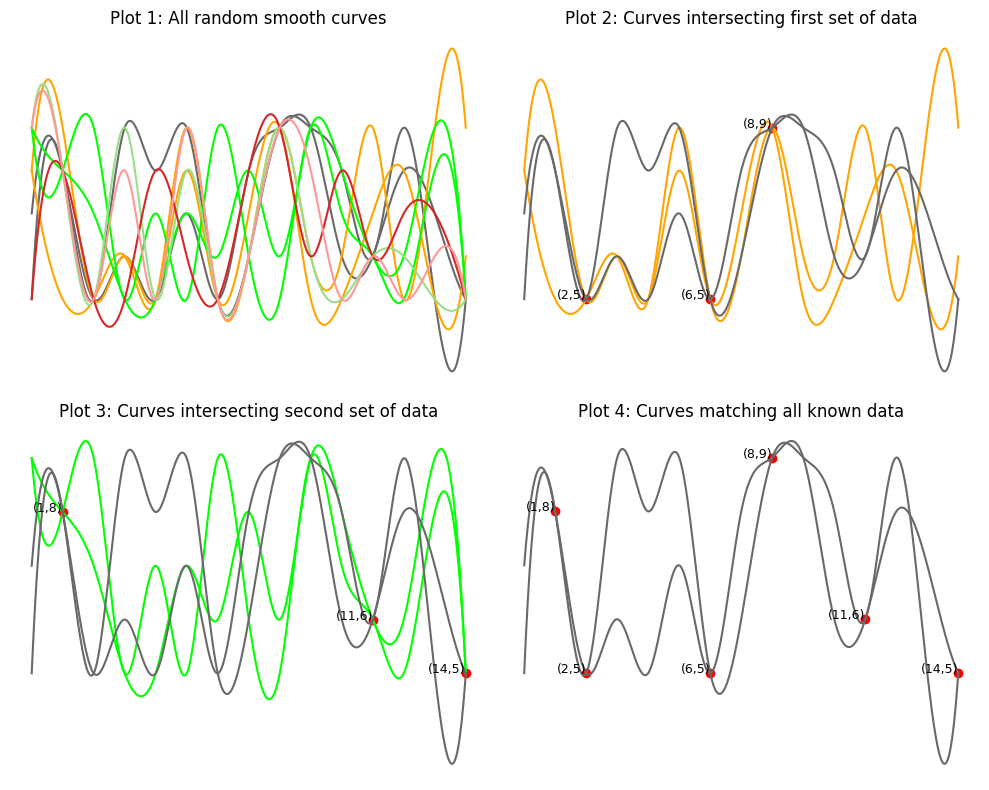
\includegraphics[width=0.9\textwidth]{plots.png}
    \caption{Smooth curves representing}
    \label{Fig:gp-curves}
\end{figure}

The \cref{Fig:gp-curves} provides a (flawed) illustration to build intuition. Plot 1 describe a large set of random smooth curves. Plot 2 shows
curves that match the first set of data, reducing the number of possible curves. Plot 3 shows curves matching
a different set of known data. Finally plot 4 shows the curves that match all of data. Notice that 
the curves in plot 4 can also be found in plot 2 and 3. This is a visual representation of how Gaussian process
gives consistent answers for different data - the set of possible curves gets restricted with data, but all
considered sets of data include the curves consistent with other sets of data. In actuality the GP doesn't 
deal with any particular function but a probability distribution of functions.

The VMBC algorithm uses GP-based Bayesian quadrature to solve the marginal likelihood. The GP-model provides a prior for the possible
functions and the Bayesian quadrature or Bayesian Monte Carlo is used for active sampling\cite{acerbi2018}. According to Rasmussen and Ghahramani, Bayesian Monte Carlo
starts with a prior over some function and makes inferences about it from a set of samples \cite{bayesian_mc}. 

The Bayesian quadrature used by the VMBC differs from standard simple methods by the sampling method. The sampling minimizes the
KL divergence and variance of the final estimate of ELBO or the evidence lowerbound. 
The minimizing is done by the acquisition function, which aims to 
minimize the uncertainty for the current posterior and for potential locations of future posteriors.\cite{acerbi2018}

\chapter{pyVMBC examples}
\label{chapter:layout}

The aim of this chapter is to provide a comprehensive yet simple usage example of the pyVMBC package. Using this

\chapter{Conclusions}
\label{chapter:conclusions}

TODO

% STEP 5: Uncomment the following lines and set your .bib file and
% desired bibliography style to make a bibliography with BibTeX.
% Alternatively you can use the thebibliography environment if you want
% to add all references by hand.
% 
\cleardoublepage %fixes the position of bibliography in bookmarks
\phantomsection

\renewcommand\bibname{References}
\addcontentsline{toc}{chapter}{\bibname} % This lines adds the bibliography to the ToC 
\bibliographystyle{abbrv} % numbering alphabetic order 
\bibliography{UH_DS_references}


\end{document}
